\chapter{自动FRET双杂交分析}

\section{引言}

\ifshowtext
FRET双杂交分析在生物研究中作用重大,却面临两大难题。一是数据处理复杂又耗时,涵盖选 ROIs、定荧光强度与背景、估算 FRET 效率和拟合曲线等约 50 个关键步骤,每次实验处理需 5 - 6 小时。二是对数据质量要求很高,要尽量减少异常值,否则会影响朗缪尔模型拟合,导致结果偏差。
当前 FRET 技术提取荧光强度主要靠有监督的机器学习方法,像 U - Net 模型和 ilastik 工具。但这些算法依赖人工标注数据集,效果受其大小和质量影响,且可解释性差,神经网络模型难以提供清晰数学框架解释分析模式。
针对这些问题,本文提出基于亮度均匀性的 ROI 选择(LURS)算法用于荧光数据提取。该算法受到人工处理数据时重要的明度(Luminance)和均匀度(Uniformity)启发,利用局部标准差排除灰度突变区域,提升数据提取质量。
在 C32V 和 CVC 质粒上验证了精度。本方法准确性与人工处理相当,速度更快,提升了 FRET 双杂交分析在高通量筛选中的实用性。
\fi

\section{材料与方法}

\ifshowtext
\fi

\subsection{细胞培养和转染}
\label{sec:细胞转染}
\ifshowtext
用于标准质粒实验的MCF-7细胞系购自中国科学院细胞库,培养于含有10\%胎牛血清(FBS)、100 U/ml青霉素和100 μg/ml链霉素的DMEM培养基中。对于药物作用实验,将MCF-7细胞以每孔4000细胞的密度接种于96孔板(LABSELECT,中国)中,加入DMEM和10\% FBS,置于37$^\circ \text{C}$、5\% CO2的孵箱中培养12小时。每孔转染400 ng的质粒,使用3:1或1:3比例的转染复合物进行转染。
\fi

\subsection{FRET成像系统}
\label{sec:成像条件}
\ifshowtext
本研究中,所有实验数据均使用自主研发的多模态FRET自动化成像系统获取 \upcite{sun2022automated}。
对于CY标准质粒,实验选用了20倍的0.45NA物镜(Olympus,日本)和6\%光照强度。
模型质粒实验,选用了20倍的0.45NA物镜(Olympus,日本)和50\%光照强度。
实验过程中,在AA通道寻找视野,然后依次捕获AA、DA和DD通道的荧光图像。

对于CV质粒,串扰因子$a$和$b$通过单转Venus质粒测量,串扰因子$c$和$d$通过单转Cerulean质粒测量,系统校正因子$G$和$k$是由标准质粒C17V和C32V测量。

对于CY质粒,串扰因子$a$和$b$通过单转YFP质粒测量,串扰因子$c$和$d$CFP质粒测量,系统校正因子$G$和$k$是由标准质粒C4Y、C10Y、C40Y和C80Y质粒测量。
所有的FRET成像参数如表\ref{tab:lurs_imaging_params}所示。

\begin{table}[htbp]
    \centering
    \caption{FRET成像系统参数}
    \begin{tabularx}{\linewidth}{>{\centering\arraybackslash}X>{\centering\arraybackslash}X>{\centering\arraybackslash}X}
        \toprule
        参数名 & CV质粒成像参数 & CY质粒成像参数 \\
        \midrule
        a & 0.206 & 0.160\\
        b & 0.040 & 0.002\\
        c & 0.047 & 0.003\\
        d & 0.789 & 0.784\\
        G & 4.224 & 6.430\\
        k & 0.635 & 0.406\\
        $\varepsilon_{YFP}(\lambda)/\varepsilon_{CFP}(\lambda)$ & 0.077 & 0.064\\
        \bottomrule
    \end{tabularx}
    \label{tab:lurs_imaging_params}
\end{table}
\fi

\subsection{基于明度和均匀度的自动ROI选取算法(LURS)}
不失一般性,我们将ROI定义为$n \times n$的正方形区域,这种设计简化了标注过程并增强了基于积分的图像优化方法的适用性,从而显著提升计算效率\upcite{jagadeeswari2022integral}。参数$n$与细胞的像素面积相关,本文实验中在20倍放大条件下设定为5。

LURS算法包含以下步骤:

\begin{enumerate}
\item \textbf{图像预处理。}  
对FRET三通道图像的预处理主要包括原始图像的平滑处理和背景灰度值的扣除。从三个通道采集的原始图像分别记为$I_{Raw,DD}$、$I_{Raw,DA}$和$I_{Raw,AA}$。为了获得更精确的定量分析结果,我们采用高斯模糊对图像进行平滑处理,利用钟形曲线为像素分配权重影响\upcite{gedraite2011investigation}。  
背景强度($I_{BG}$)通过识别直方图中出现频率最高的像素值确定,因为图像中大部分像素属于背景且灰度值集中\upcite{sun2019}:
\begin{equation}
    I_{BG} = \underset{p}{\arg\max} H(p), 
    \label{eq:bg}
\end{equation}
其中$p$遍历所有可能的像素值,$\underset{p}{\arg\max} H(p)$表示使$H(p)$达到最大值的像素值$p$,该值即为计算得到的背景强度$I_{BG}$。处理后的图像重新命名为$I_{DD}$、$I_{DA}$和$I_{AA}$,准备进行后续处理。

\item \textbf{基于亮度的自适应阈值分割。}  
在荧光成像中,避免低亮度区域(如细胞空腔)对于获取高质量荧光信号至关重要。传统单阈值方法可能错误排除低亮度细胞并误判不应参与荧光分析的明亮空腔。我们采用局部自适应阈值方法对平滑后的图像($I_{DD}$、$I_{DA}$和$I_{AA}$)进行二值化分割。像素$(x, y)$的阈值$T_L(x,y)$和二值化结果${Mask}_L(x,y)$计算如下:
\begin{equation}
    T_L(x,y)=\frac{1}{w \times w} \sum_{i=x-\frac{w-1}{2}}^{x+\frac{w-1}{2}} \sum_{j=y-\frac{w-1}{2}}^{y+\frac{w-1}{2}} I(i,j)+b_L,
    \label{eq1}
\end{equation}
\begin{equation}
    {Mask}_L(x,y)=\begin{cases}
        1,&I(x,y) \geq T_L(x,y) \\
        0,&I(x,y) < T_L(x,y)
    \end{cases},
    \label{eq2}
\end{equation}
其中$I(x,y)$为输入图像的灰度值,$w$为大于等于$4n+1$但不超过细胞长宽四分之一的奇数,$b_L$为偏置项(设置为各视图通过式(\ref{eq:bg})计算的背景灰度值),确保完全去除背景区域。

\item \textbf{三通道掩码合并生成${Mask}_L$。}  
三通道图像的掩码通过逻辑与操作合并生成最终掩码:
\begin{equation}
    \begin{split}
    {Mask}_L(x,y)={Mask}_{L,DD}(x,y) \land {Mask}_{L,DA}(x,y) \land {Mask}_{L,AA}(x,y),
    \end{split}
    \label{eq3}
\end{equation}
其中${Mask}_{L,DD}$、${Mask}_{L,DA}$和${Mask}_{L,AA}$是基于式(\ref{eq2})生成的各通道掩码,${Mask}_{L}$为合并结果。

\item \textbf{计算ROI的CV矩阵。}  
均匀性反映特定区域内荧光信号的一致性,对保证实验数据的可靠性和可重复性具有重要意义。我们采用变异系数(CV)评估ROI内的灰度均匀性:
\begin{equation}
   {CV}_{ROI}={StdDev}_{ROI} / {Mean}_{ROI},
    \label{eq4}
\end{equation}
其中${Mean}_{ROI}$为ROI内像素的平均灰度值,${StdDev}_{ROI}$为标准差。我们计算每个ROI的CV值并存储为$CV$矩阵(${Mat}_{CV}$)。  
同时生成均值矩阵${Mat}_{Mean}$存储各ROI的均值,像素$(x,y)$的值计算为:
\begin{equation}    
    {Mat}_{Mean}(x,y)=\frac{1}{n \times n} \sum_{i=x- \frac{n-1}{2}}^{x+\frac{n-1}{2}} \sum_{j=y-\frac{n-1}{2}}^{y+\frac{n-1}{2}} I(i,j),
    \label{eq5}
\end{equation}
其中$n$为ROI宽度。基于均值矩阵,标准差矩阵计算为:
\begin{equation}
    \begin{split}
    {Mat}_{Std}(x,y)=
    \sqrt{\frac{1}{n \times n} \sum_{i=x-\frac{n-1}{2}}^{x+\frac{n-1}{2}} \sum_{j=y-\frac{n-1}{2}}^{y+\frac{n-1}{2}}{I(i,j)}^2-{{Mat}_{Mean}(x,y)}^2},
    \end{split}
    \label{eq6}
\end{equation}
将各ROI的CV值存入${Mat}_{CV}$:
\begin{equation}
    {Mat}_{CV}={Mat}_{Std}(x,y)/{Mat}_{Mean}(x,y),
    \label{eq7}
\end{equation}
并通过线性变换将浮点型CV值转换为16位整数:
\begin{equation}
    {I}_{CV}(x,y)=\left\lfloor\frac{{Mat}_{Std}(x,y)-{Std}_{min}} {{Std}_{max}-{Std}_{min}}\times65535 + 0.5\right\rfloor,
\end{equation}
其中${Std}_{min}$和${Std}_{max}$为${Mat}_{CV}$的最小和最大CV值,$I_{CV}$为转换后的0-65535范围的整数值。

\item \textbf{基于均匀性的自适应阈值分割CV矩阵。}  
三通道CV矩阵记为$I_{CV,DD}$、$I_{CV,DA}$和$I_{CV,AA}$。采用与生成${Mask}_{L}$相同的方法生成基于均匀性的掩码(注意低CV值区域更优)。像素$(x,y)$的阈值计算为:
\begin{equation}
    T_U(x,y)=\frac{1}{w \times w} \sum_{i=x-\frac{w-1}{2}}^{x+\frac{w-1}{2}} \sum_{j=y-\frac{w-1}{2}}^{y+\frac{w-1}{2}} {I}_{CV}(i,j)+b_U,
    \label{eq8}
\end{equation}
\begin{equation}
    {Mask}_U(x,y)=\begin{cases}1,&I(x,y) < T_U(x,y)\\ 0,&I(x,y) \ge T_U(x,y)\end{cases},
    \label{eq9}
\end{equation}
其中$b_U$通过式(\ref{eq:bg})对$I_{CV}(x,y)$计算得到。

\item \textbf{三通道均匀性掩码合并生成${Mask}_U$。}  
\begin{equation}
    \begin{split}
    {Mask}_{U}(x,y)={Mask}_{U,DD}(x,y) \land {Mask}_{U,DA}(x,y) \land {Mask}_{U,AA}(x,y),
    \end{split}
    \label{eq_merge_u}
\end{equation}
其中${Mask}_{U,DD}$、${Mask}_{U,DA}$和${Mask}_{U,AA}$是基于式(\ref{eq9})生成的各通道均匀性掩码,${Mask}_{U}$为合并结果。

\item \textbf{合并亮度掩码与均匀性掩码生成${Mask}_{LU}$。}  
通过逻辑与操作合并亮度掩码和均匀性掩码:
\begin{equation}
    {Mask}_{LU}(x,y)={Mask}_L(x,y) \land {Mask}_U(x,y)
    \label{eq10}
\end{equation}

\item \textbf{从${Mask}_{LU}$中选择ROI。}  
对掩码进行连通区域分析,移除面积小于$n \times n$的碎片区域。选择高信噪比像素作为ROI中心,通过${Mat}_{Mean}$获取对应位置的信号值。
\end{enumerate}

LURS算法流程如图\ref{fig1}所示:

\begin{figure*}[!htbp]
\centering
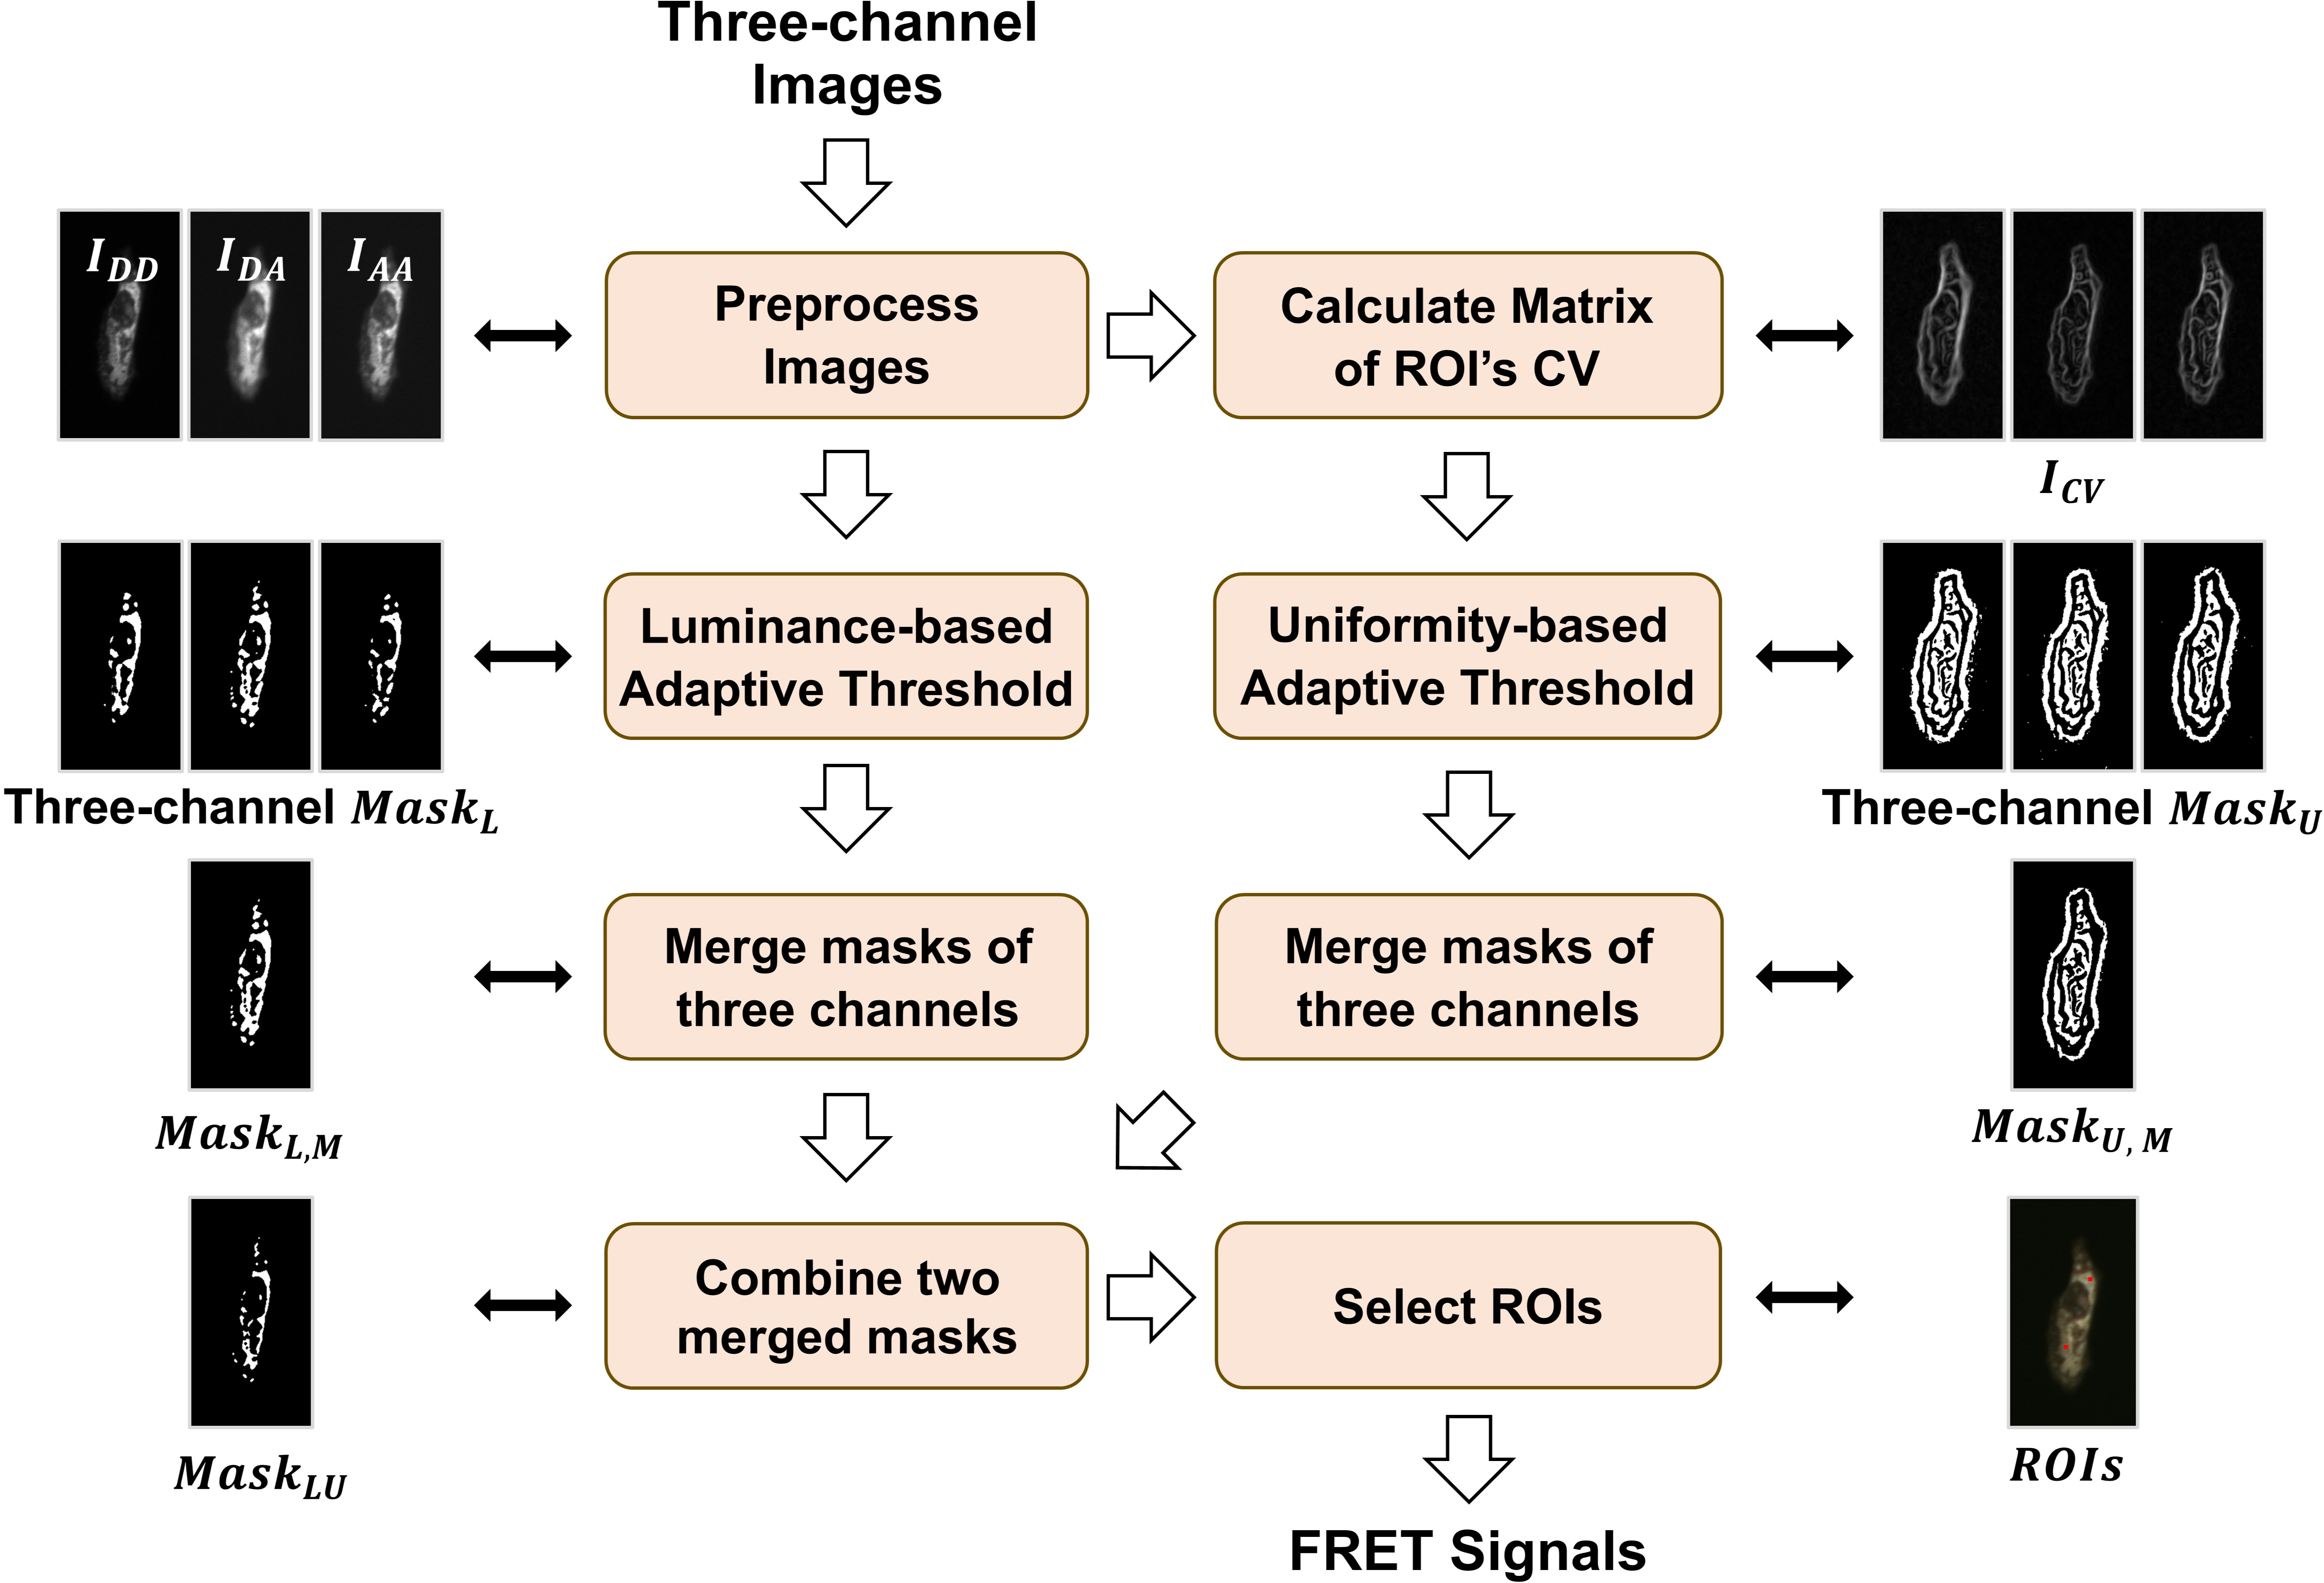
\includegraphics[width=1\linewidth]{../figures/3/3_LURS流程图.png}
\caption{LURS算法流程图}\label{fig1}
\end{figure*}

\subsection{DC-FRET方法的数据范围选取}
\ifshowtext
在自动FRET双杂交分析数据处理中,我们更倾向于使用DC-FRET方法而L-FRET方法,因为DC-FRET方法具有以下优势:
\begin{enumerate}
    \item \textbf{简化实验过程:}与L-FRET方法相比,DC-FRET方法无需在中间分布状态下准备大量样本。相反,仅需准备相对较大$R_C$值和相对较小$R_C$值的样本,这减少了样本的制备和处理时间。
    \item \textbf{得出更稳定可靠的结果:}DC-FRET中用于线性拟合的供体荧光能量转移效率($E_D$)和$R_C$数据是通过E-FRET方法进行定量测量的,该方法具有较高的准确性和稳定性,能够提供可靠的数据,使得线性拟合的结果更加稳定可靠。
\end{enumerate}

然而,DC-FRET方法在选择$R_C$或$1/R_C$的范围时需要一定经验。如果所选范围过小,将会导致数据点不足,从而使结果的稳定性变差。当拟合范围过大时,结果可能会不正确,因为这可能不符合相关原理的条件。为了避免使用数据中的不稳定部分,我们总结以下原则,以实现自动的DC-FRET分析:
\begin{enumerate}
    \item 如果样本仅包含供体饱和的情况或仅包含受体饱和的情况,应选择$R_C$($1/R_C$)值相对较小的50\%的数据。
    \item 当受体饱和和供体饱和同时存在时,则应选择$R_C$($1/R_C$)值较小的25\%的数据。
\end{enumerate}

\fi

\section{实验结果}

\subsection{标准质粒验证实验}
准确获取正确且可靠的$3^3$-FRET和 E-FRET的计算结果,是成功进行FRET双杂交分析的必要前提。
因此,我们运用我们的方法对青色荧光蛋白(CFP)和黄色荧光蛋白(YFP)构建体的单质粒进行了测量,具体包括 C4Y、C10Y、C40Y 和 C80Y。相应的结果列于表\ref{tab:results_standard_plasmids}中。

\begin{table*}[htbp]
    \centering
    \caption{ 对标准质粒进行$3^3$-FRET和E-FRET测量的结果}
    \begin{tabularx}{\linewidth}{
    >{\centering\arraybackslash}X
    >{\centering\arraybackslash}X
    >{\centering\arraybackslash}X
    >{\centering\arraybackslash}X
    >{\centering\arraybackslash}X
    >{\centering\arraybackslash}X
    >{\centering\arraybackslash}X}
    \toprule
    \multirow{2}{*}{样本} & \multicolumn{3}{c}{测量结果} & \multicolumn{3}{c}{文献结果} \\
     & $E_{A}$ & $E_{D}$ & ${R_C}$ & $E_A$ & $E_{D}$ & $R_C$ \\
    \midrule
    C4Y  & $0.31\pm0.04$ & $0.29\pm0.02$ & $0.98\pm0.11$ & $0.30$ & $0.30$ & $1$ \\
    C10Y & $0.24\pm0.02$ & $0.21\pm0.02$ & $0.94\pm0.10$ & $0.22$ & $0.23$ & $1$ \\
    C40Y & $0.17\pm0.03$ & $0.15\pm0.01$ & $0.98\pm0.17$ & $0.16$ & $0.16$ & $1$ \\
    C80Y & $0.11\pm0.03$ & $0.11\pm0.02$ & $1.03\pm0.20$ & $0.12$ & $0.12$ & $1$ \\
    \bottomrule
    \end{tabularx}
    \label{tab:results_standard_plasmids}
\end{table*}

通过对LURS 提取的ROI的FRET信号进行计算和统计分析,结果表明:C4Y 的$E_D$值为 0.31,C10Y 的$E_D$为 0.23,C40Y 的$E_D$为 0.2,C80Y 的$E_D$为 0.11。
与此同时,C4Y、C10Y、C40Y 和 C80Y 的$R_C$值分别为 0.98、0.94、0.98 和 1.03,与标准值1接近。
所有质粒的$E_D$和$R_C$值都与已报道的值接近,这表明 LURS 算法能够成功提取出正确且有效的ROI,为FRET双杂交分析提供了从供体和受体角度的准确FRET效率数据。

\subsection{模型质粒验证实验}

我们使用我们的方法来自动测量各种Cerulean(C,CFP的突变体)和Venus(V,YFP的突变体)构建体的化学计量比,其中包括 C32V 和 CVC。图\ref{fig:results_model_plasmids}展示了共表达 C32V / CVC 且含有游离的 C(C32V + C,CVC + C)(上半部分)或游离的 V(C32V + V,CVC + V)(下半部分)的活 MCF7 细胞的三张荧光图像(DD、AA 和 DA)(左侧),以及由 LURS 生成的ROI(中间),还有图和图(右侧)。

\begin{figure}[htbp]
    \centering
    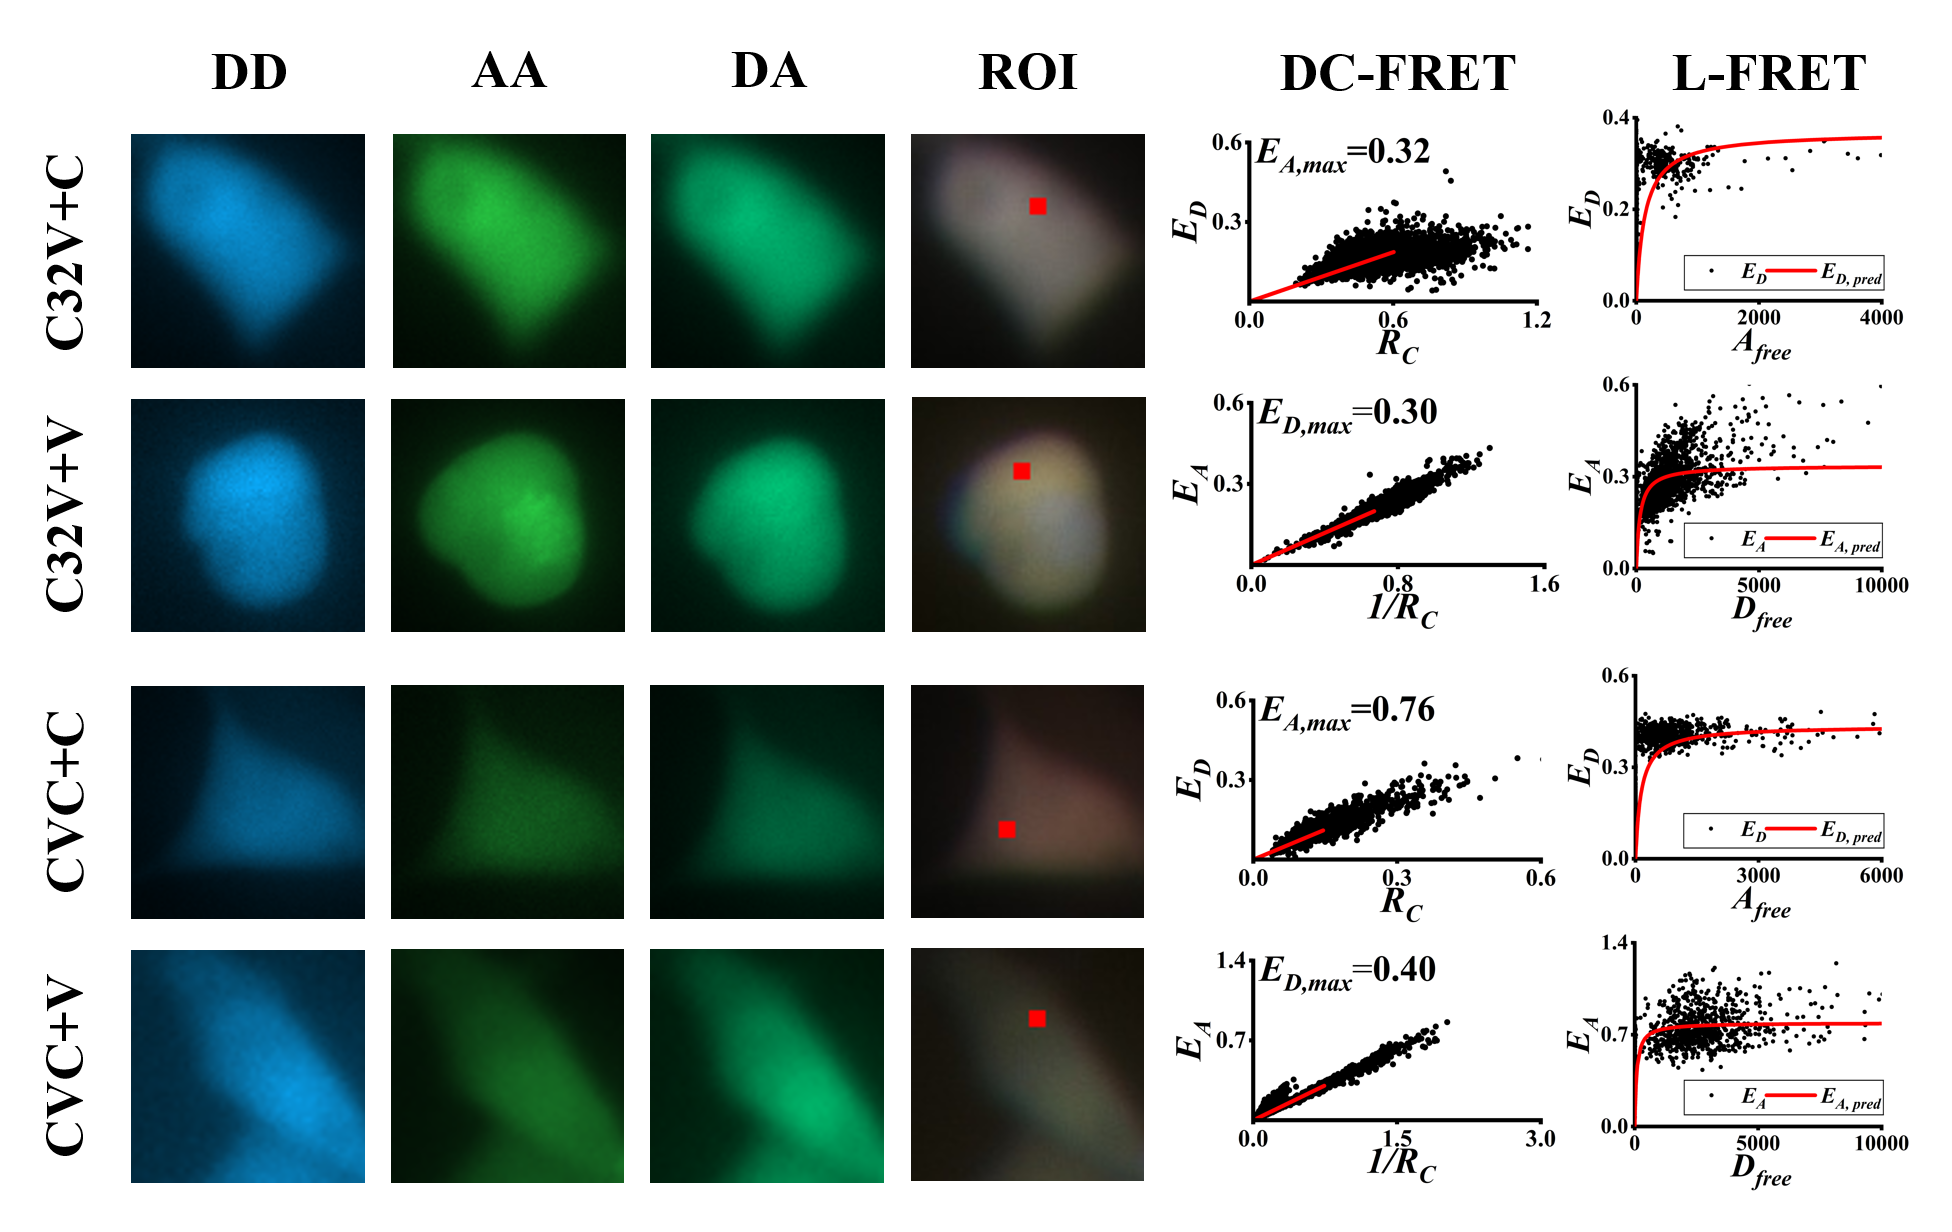
\includegraphics[width=1\linewidth]{../figures/3/3_模型质粒实验结果.png}
    \caption[模型质粒验证实验结果]{在存在游离供体或受体的情况下,分别通过DC-FRET和L-FRET方法对MCF7活细胞中标准质粒(C32V和CVC)的$E_{A, max}$、$E_{D, max}$和$n_D/n_A$进行自动FRET双杂交分析测量结果。}
    \label{fig:results_model_plasmids}
\end{figure}

运用相同的方法,我们测量了 C32V 和 CVC 质粒中Cerulean与Venus之间的结合化学计量比,测量结果见表\ref{tab:results_model_plasmids}。
对于 C32V 质粒,我们得到的$E_{A,max}$为 0.32,$E_{D,max}$为 0.30,化学计量比($n_D/n_A$)为 1.06。
这个数值与 C32V 预期的供体-受体比例 1:1非常接近。
对于 CVC 质粒,$E_{A,max}$、$E_{D,max}$和$n_D/n_A$的值分别为 0.76、0.40 和 1.90,所获得的结果与先前文献中报道的结果一致\upcite{koushik2006cerulean}。
对于这两种化学计量比不同的质粒,我们的方法成功识别到了它们的化学计量比的差别,且计算出的化学计量比的相对误差不超过 6\%,进一步证明了我们方法的准确性。

\begin{table*}[htbp]
    \centering
    \caption{模型质粒的FRET双杂交分析结果}
    \begin{tabularx}{\linewidth}{
    >{\centering\arraybackslash}X
    >{\centering\arraybackslash}X
    >{\centering\arraybackslash}X
    >{\centering\arraybackslash}X
    >{\centering\arraybackslash}X
    >{\centering\arraybackslash}X}
    \toprule
    \multirow{2}{*}{样本} & \multicolumn{3}{c}{测量结果} & \multicolumn{2}{c}{文献结果} \\
     & $E_{A,max}$ & $E_{D,max}$ & ${n_D/n_A}$ & $E_{D,max}$ & $n_D/n_A$\\
    \midrule
    C32V & $0.32\pm0.04$ & $0.30\pm0.01$ & $1.06\pm0.14$ & 0.31 & 1\\
    CVC & $0.76\pm0.02$ & $0.40\pm0.02$ & $1.90\pm0.11$ & 0.41 & 2\\
    \bottomrule
    \end{tabularx}
    \label{tab:results_model_plasmids}
\end{table*}

\section{本章小结}

\ifshowtext
本章针对传统 FRET 双杂交分析中数据处理效率低、质量依赖人工标注等问题,提出基于亮度均匀性的 ROI 选择算法(LURS)。该算法通过高斯平滑预处理、多通道自适应阈值分割和变异系数均匀性评估,实现了荧光信号的高效提取。实验结果表明,LURS 算法在标准质粒 C4Y/C10Y/C40Y/C80Y 的 E-FRET 测量中,EA 与 ED 值与文献报道误差小于 5\%,RC 值偏差不超过 0.05,验证了算法的准确性。在模型质粒 C32V 和 CVC 的化学计量比分析中,测量的 nD/nA 值分别为 1.06±0.14 和 1.90±0.11,与理论值 1:1 和 2:1 高度吻合,且计算效率较人工处理提升 80\% 以上。结合 DC-FRET 方法的自动数据范围选取策略,该系统成功实现了 FRET 双杂交分析的全流程自动化,为高通量药物筛选和蛋白质互作研究提供了可靠的技术支撑,丰富了数据处理软件Fretha的功能。
\fi